\chapter{Desarrollo de un Diseño Inicial}

Como un paso preliminar para desarrollar el diseño del MLR, fue necesario llevar a cabo un estudio de su naturaleza, teniendo en cuenta las leyes que gobiernan su comportamiento, con el fin de establecer una base teórica y desarrollar criterios requeridos durante la etapa de diseño, como en las etapas de optimización y control. Una vez esta base teórica ha sido definida, se procede a la proposición de un diseño inicial orientado a cumplir los requisitos del motor lineal.

El desarrollo de este estudio abarca diferentes áreas del electromagnetismo y las máquinas eléctricas, por lo que, con el fin de enfocar el contenido principal del libro en los puntos claves del diseño y en los resultados, las bases teóricas y herramientas de cálculo se han movido al apéndice B para el lector interesado, mientras que en este capítulo se muestra únicamente el proceso de diseño basado en las ecuaciones y relaciones que se derivan en este apéndice, los resultados obtenidos y discusiones sobre los mismos.

\section{Descripción del MLR}
En el capítulo anterior se seleccionó el MLR para cumplir los requisitos del diseño. Dentro de los MLR, existen varias configuraciones que pueden utilizarse, cuyas diferencias se encuentran principalmente en la geometría del secundario, ya que para el primario se usa un devanado distribuido de tres fases. Por el lado del secundario, con el fin de incrementar el coeficiente de saliencia en los MLR, se han propuesto diferentes topologías, tales como laminaciones segmentadas \cite{lawrenson1967} y el secundario axial laminado anisotrópico (ALA) \cite{cruickshank1966,hamler1998,kostko1923,leekimlee2014}, el cual fue utilizado para el motor diseñado.

El proceso de diseño contempla la especificación de parámetros físicos y eléctricos del mismo. Su geometría se muestra simplificada en dos dimensiones como una vista lateral en la Fig. \ref{fig:LVRMdi}. El primario consta de un núcleo de material ferromagnético y un devanado trifásico distribuido. El secundario consta de grupos de laminaciones que abarcan una distancia igual a un paso polar $\tau$. Estos conjuntos pueden contener de 4 a más laminaciones \cite{boldea2013}. La región entre el primario y el secundario se conoce como el \textbf{entrehierro}.

\begin{figure}[tb]
\centering
\includegraphics[scale=0.8]{../img/Desarrollo_de_un_diseno_inicial/LVRM.png}
\caption{Geometría del MLR}
\label{fig:LVRMdi}
\end{figure}

Desde el punto de vista de la geometría, los parámetros de diseño son el paso polar, el área de las ranuras, dada por las longitudes $b_s$ y $h_s$, la distancia $g$ del entrehierro, la geometría de los dientes del primario, la altura $h_c$ de la región del primario sobre la cual se encuentra el devanado, el número de laminaciones en el secundario y su grosor (véase la Fig. \ref{fig:primaryreactionrail}). Además de calcular estos parámetros, es necesario determinar las especificaciones del devanado como su distribución y el número de vueltas. Por último, desde el punto de vista eléctrico, deben calcularse los valores de operación nominal del motor para el voltaje de entrada y la corriente de fase.

\begin{figure}[b]
    \centering
    \begin{subfigure}[b]{0.49\textwidth}
        \includegraphics[width=\textwidth]{../img/Desarrollo_de_un_diseno_inicial/primary.PNG}
        \caption{Geometría del primario}
        \label{fig:primary}
    \end{subfigure}
    ~ %add desired spacing between images, e. g. ~, \quad, \qquad, \hfill etc. 
      %(or a blank line to force the subfigure onto a new line)
    \begin{subfigure}[b]{0.49\textwidth}
        \includegraphics[width=\textwidth]{../img/Desarrollo_de_un_diseno_inicial/reactionrail.PNG}
        \caption{Geometría del secundario}
        \label{fig:reactionrail}
    \end{subfigure}
    \caption{Detalle de las geometrías del primario y el secundario en el MLR.}\label{fig:primaryreactionrail}
\end{figure}

El análisis de las máquinas eléctricas usualmente inicia con la suposición de que la reluctancia en la dirección del movimiento es constante. Esto se traduce en que la inductancia del motor es constante independiente de la posición relativa entre el primario y el secundario \cite{chapman2003}. El MLR, al contrario, está específicamente diseñado para que la inductancia sea una función de la posición relativa entre el primario y el secundario, por lo que la suposición de la reluctancia constante no es aplicable, por lo que se aplica la transformación de Park (véase el apéndica A) para expresar las variables electromagnéticas del motor en términos de los ejes directo y en cuadratura.

\section{Requerimientos del motor}
El problema considerado consiste en diseñar un MLR capaz de producir una potencia mecánica de salida de 100 W. Las especificaciones de empuje del motor pueden ser determinadas al especificar valores de aceleración $a$ y la masa total de la parte móvil (incluyendo la carga del motor) $m$. Estas especificaciones fueron calculadas asumiendo aceleración inicial constante y fricción despreciable.
Teniendo en cuenta una carga de 2 kg y estimando inicialmente una masa de 2 kg para el primario, la masa total del móvil es de 4 kg. Se escogió una velocidad promedio $v_f$ de 2 m/s, de forma que, dada una potencia mecánica de 100 W, se requiere un empuje promedio de 50 N. El empuje pico es responsable de llevar el motor de velocidad cero a la velocidad promedio de 2 m/s, y fue calculado tomando 100 W de potencia como el límite máximo del motor. Si $t_f$ es el tiempo de aceleración, la siguiente relación puede establecerse:
\begin{equation*}
P = 100\text{ W} =
\frac{2v_f^2}{t_f}
\end{equation*}
De esta forma, teniendo en cuenta los valores conocidos, se obtiene un tiempo de aceleración de 80 ms y una aceleración es 15 m/s$^2$. Con estos valores, las especificaciones de empuje del motor pueden resumirse como un empuje promedio $F_x$ y un empuje pico $F_{xmax}$ como
\begin{align*}
F_x &= 50\text{ N}\\
F_{xmax} &= 100\text{ N}
\end{align*}
Es necesario notar que la estimación de una masa total del móvil impone una limitación en el tamaño del primario, el cual depende del paso polar y el ancho del motor.

\section{Descripción del proceso de diseño}
El enfoque utilizado para obtener el diseño inicial se basó en resultados numéricos, como los mostrados en \cite{boldea1994}, relaciones analíticas encontradas en la teoría de los motores lineales \cite{boldea2013, gieras2000} y consideraciones empíricas. La base teórica para el diseño, así como la derivación de varias de las fórmulas utilizadas durante el proceso del diseño, se muestran en el apéndice B. 

El proceso de diseño se puede resumir en 4 etapas, como se muestra en el diagrama de flujo mostrado en la Fig. \ref{fig:flujodiseno} (las fuerzas magnetomotrices se indican como \textit{fmms}). Estos pasos se desarrollan a continuación.

\begin{figure}[t]
\centering
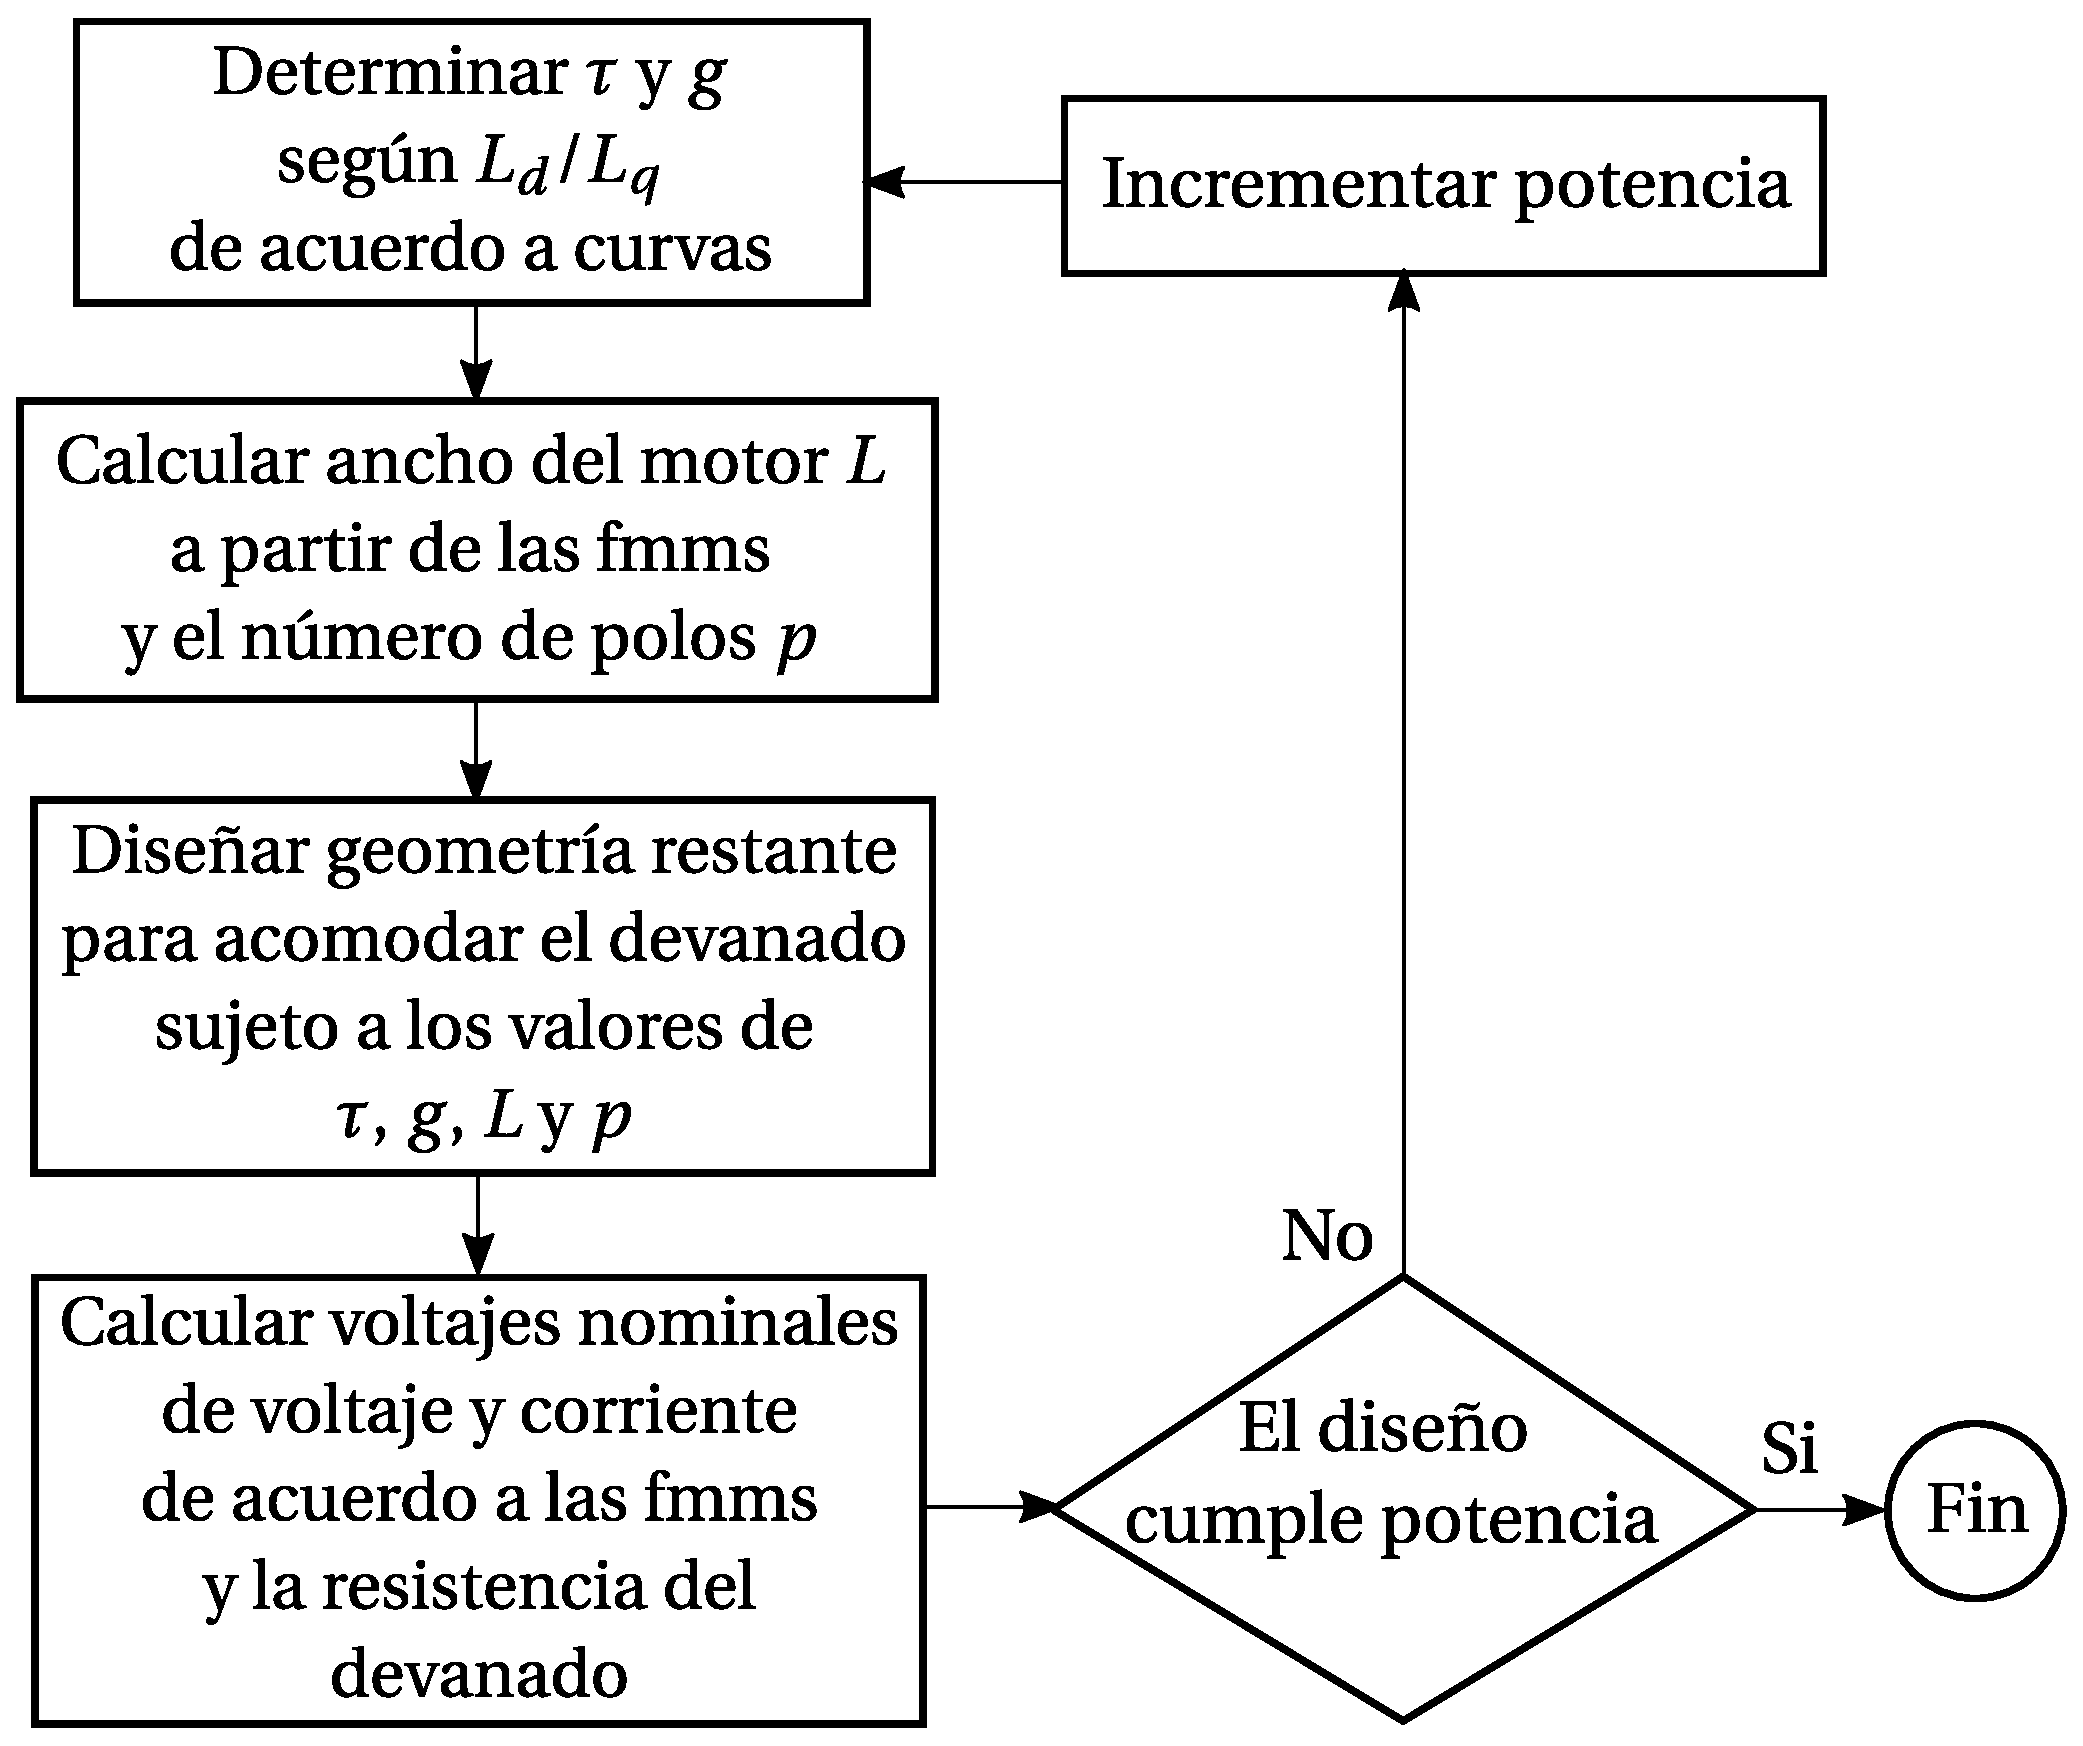
\includegraphics[scale=0.3]{../img/Desarrollo_de_un_diseno_inicial/flujodiseno.eps}
\caption{Pasos del proceso de diseño}
\label{fig:flujodiseno}
\end{figure}

\subsection{Determinación de $\tau$ y $g$}
El objetivo principal al diseñar un MLR es maximizar la razón entre la inductancia del eje directo y la inductancia en el eje en cuadratura $L_d/L_q$. Existen dos variables del MLR en particular que tienen un efecto en esta razón: el paso polar y la distancia del entrehierro \cite{boldea1994}, como  se concluyen de los resultados mostrados en \cite{boldea1994} y del que se obtienen un par de curvas que permiten seleccionar un valor de $\tau$ y $g$ para obtener un valor dado de la razón $L_d/L_q$ (véase la sección A.3 del apéndice B para más detalles sobre estas curvas).

Con el fin de obtener un valor alto y razonable de $L_d/L_q$, se escogió una distancia del entrehierro de 0.5 mm y un paso polar de 3.5 cm. Estos valores indican, de acuerdo a las curvas mencionadas anteriormente, una razon $L_d/L_q$ igual a 3.63.

\subsection{Cálculo del ancho del motor}
Como se sugiere en \cite{boldea2013}, se asumió un valor práctico de 0.4 T para la densidad de flujo magnético pico en el entrehierro, con el fin de encontrar la densidad de flujo magnético pico en el eje directo $B_{epd}$ por medio de la ecuación A.35. 
Las fuerzas magnetomotrices en los ejes directo y en cuadratura se definen como $W_1 I_d$ y $W_1 I_q$, donde $W_1$ es el número de vueltas por fase, $I_d$ es la componente de la corriente de fase en el eje directo e $I_q$ es la componente en el eje en cuadratura.

Utilizando las ecuaciones de inductancia y empuje, se obtiene una sola ecuación donde son variables el número de polos y el ancho del motor. Al fijar un número de polos igual a 4 (teniendo en cuenta las consideraciones de tamaño mencionadas anteriormente), queda determinado el ancho del motor, con un valor de 7.15 cm.

De acuerdo al procedimiento anterior, se concluye que el método utilizado basa la determinación de la razón $L_d/L_q$ en tres variables, principalmente: el paso polar, la distancia del entrehierro y el ancho del motor.

\begin{figure}[!]
\centering
\rotatebox{90}{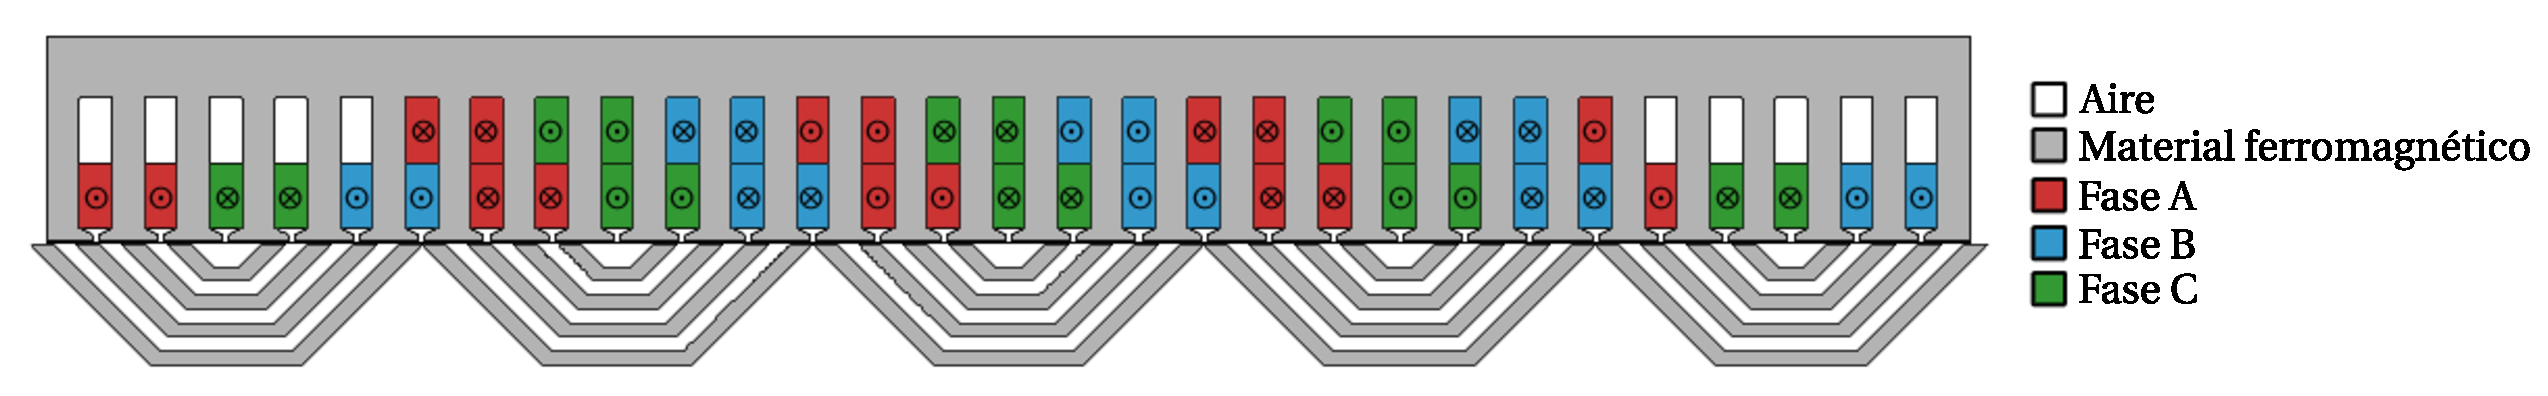
\includegraphics[width=1.40\linewidth]{../img/Desarrollo_de_un_diseno_inicial/domains.eps}}
\caption{Geometría del MLR diseñado, mostrando el primario en su totalidad.}
\label{fig:domains}
\end{figure}


\subsection{Diseño de la geometría restante}
Con el fin de reducir los armónicos en el flujo en el entrehierro y producir una distribución del campo aproximadamente senoidal, se decidió utilizar un devanado distribuido de doble capa \cite{chapman2003}, donde la razón entre el paso de bobina $y$ y el paso polar $\tau$ es $y/\tau=5/6$ y el número de ranuras por polo por fase es $q = 2$. De esta forma, el paso de ranura es
\begin{equation}
\tau_s = \frac{\tau}{3q}
\end{equation}
debido a que el devanado es de tres fases. Como se sugiere en \cite{boldea2013}, se seleccionaron posteriormente los parámetros $b_s$ y $h_s$ como
\begin{align*}
b_s &= 3\tau_s/4\\
h_s &= 3b_s
\end{align*}
La altura $h_c$ se calculó de forma que se redujera la saturación en el núcleo cuando la densidad de flujo magnético en el entrehierro tiene su valor máximo, de acuerdo a las relaciones mostradas en \cite{boldea2010}. El número de ranuras fue determinado por la ecuación A.32, obteniéndose en total 29 ranuras.
Con respecto al secundario, se decidió trabajar con 4 laminaciones, que producen un ancho $w_c$ de 3 mm. Un mayor número de laminaciones produciría grosores más bajos que harían el secundario más difícil de fabricar y más propenso a la saturación. Así queda determinada completamente la geometría del MLR, como se muestra en la Fig. \ref{fig:domains}. En esta figura, el lado de una bobina entrando a la página se muestra con el símbolo $\otimes$, y el lado saliendo se muestra con el símbolo $\odot$.

\subsection{Cálculo de voltajes y corrientes nominales}
La resistencia $R_s$ del primario fue calculada de acuerdo a su geometría y asumiendo que el material utilizado es cobre.

Como se muestra en el apéndice B, el voltaje de fase $V_p$ del MLR puede descomponerse en sus componentes en directo $V_d$ y en cuadratura $V_q$, de forma que
\begin{equation*}
V_p = \sqrt{V_d^2 + V_q^2}
\label{phasevoltage}
\end{equation*}
En estado estacionario, estas componentes pueden expresarse como
\begin{align}
V_d &= R_s I_d - v_{me}L_q I_q\\
V_q &= R_s I_q + v_{me}L_d I_d
\label{dqssvoltages}
\end{align}
Fijando un voltaje de fase $V_p$ práctico de 45V, las ecuaciones \ref{phasevoltage} y \ref{dqssvoltages} pueden combinarse para encontrar el número de espiras del devanado, obteniéndose 422 por fase.
Una vez se tienen el número de vueltas, se calcularon las corrientes en los ejes directo y en cuadratura teniendo en cuenta las fuerzas magnetomotrices y la corriente de fase $I_a$:
\begin{align*}
I_d &= \frac{W_1 I_d}{W_1}\\
I_q &= \frac{W_1 I_q}{W_1}\\
I_a &= \sqrt{I_d^2 + I_q^2}
\end{align*}
obteniéndose un valor de 1.78 A para la corriente de fase.

\section{Estimación de la eficiencia y la masa}
La eficiencia se calcula como la razón entre la potencia mecánica de salida y la potencia eléctrica de entrada:
\begin{equation*}
\eta = \frac{F_x v}{3V_p I_a\cos\phi}
\end{equation*}
Entonces, el producto eficiencia-factor de potencia es
\begin{equation}
\eta\cos\phi = \frac{F_x v}{3V_p I_a}
\label{effpfproduct}
\end{equation}
que para un empuje $V_x$ de 50 N y una velocidad $v$ de 2 m/s (que producen una potencia mecánica de salida de 100 W), es igual a 0.424.
Por otro lado, la eficiencia también puede calcularse como la razón entre la potencia mecánica de salida y la suma entre esta potencia y las pérdidas en el cobre. Teniendo en cuenta el valor calculado para la resistencia del primario, estas pérdidas son de 85 W, por lo que la eficiencia es del 54\%. Reemplazando estos valores en la ecuación \ref{effpfproduct} y despejando $\cos\phi$, se obtiene una factor de potencia de 0.784.

Finalmente, de acuerdo al procedimiento descrito en el apéndice B, se estimó la masa del motor a partir de su geometría y las densidades del cobre y el hierro, obteniéndose una masa de 1.34 kg. Es necesario notar que este valor es bastante aproximado, ya que el núcleo del primario es laminado, y no está hecho de hierro completamente.

En la Tabla \ref{table:physicalparams} se resumen los parámetros físicos del motor, y en la Tabla \ref{table:electmechparams} sus características eléctricas y mecánicas.

\begin{table}[btp]
\centering
\caption{Parámetros físicos del diseño inicial del MLR}
\label{table:physicalparams}
\begin{tabular}{c c c}
\hline\hline\\
Símbolo & Descripción & Valor \\
\hline\\
$\tau$ & Paso polar & 3.5 cm\\
$g$ & Distancia del entrehierro & 0.5 mm\\
$y/\tau$ & Razón paso de bobina/paso polar & 5/6\\
$L$ & Ancho del motor & 7.15 cm\\
$\tau_s$ & Paso de ranura & 5.83 mm\\
$b_s$ & Ancho de ranura & 4.38 mm\\
$h_s$ & Alto de ranura & 13.13 mm\\
$h_c$ & Altura posterior del núcleo & 5.57 mm\\
$z$ & Número de ranuras en el primario & 29\\
$W_1$ & Vueltas por fase & 422\\
$L_p$ & Longitud del primario & 16.9 cm\\
$w_{rr}$ & Ancho de las laminaciones & 3 mm\\
\hline\hline\\
\end{tabular}
\end{table}

\begin{table}[btp]
\centering
\caption{Características eléctricas y mecánicas del diseño inicial del MLR}
\label{table:electmechparams}
\begin{tabular}{c c c}
\hline\hline\\
Descripción & Valor \\
\hline\\
Empuje & 50 N\\
Aceleración & 25 m/s$^2$\\
Velocidad & 2 m/s\\
Potencia mecánica & 100 W\\
Voltaje de fase & 45 V\\
Corriente de fase & 1.779 A\\
Eficiencia & 54.1\%\\
Factor de potencia & 0.784\\
\hline\hline\\
\end{tabular}
\end{table}

\section{Modelamiento y aplicación del FEM}
En el trabajo realizado, se hizo uso del software COMSOL para la aplicación del método de elementos finitos (FEM) en dos dimensiones, debido a que posee las herramientas necesarias para modelar el motor, así como diferentes materiales que permiten describir su comportamiento.

Tanto el núcleo del primario como el secundario fueron modelados utilizando una curva de magnetización lineal para tener en cuenta la saturación en estos dominios, la cual es mostrada en la Fig. \ref{fig:magdata}.

\begin{figure}[btp]
\centering
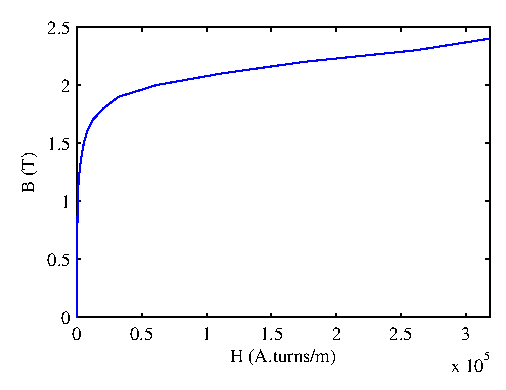
\includegraphics[scale=1]{../img/Desarrollo_de_un_diseno_inicial/magdata.eps}
\caption{Curva de magnetización utilizada en materiales ferromagnéticos.}
\label{fig:magdata}
\end{figure}

El devanado de tres fases fue modelado utilizando un dominio de bobina de múltiples vueltas, que consiste en cables aislados de cobre con baja área transversal. Como se muestra en la Fig. \ref{fig:domains}, la distribución y dirección de los devanados en cada ranura debe ser definida apropiadamente para obtener resultados consistentes.

Con respecto a la discretización del espacio, el enmallado de los dominios se realizó cuidadosamente en regiones donde los materiales son delgados, como el entrehierro \cite{bianchi2011}. Un borde de control se añadió en esta región para garantizar al menos dos capas de elementos en esta región, como se muestra en la Fig. \ref{fig:mesh}.

\begin{figure}[btp]
\centering
\includegraphics[scale=0.6]{../img/Desarrollo_de_un_diseno_inicial/mesh}
\caption{Enmallado del modelo en el entrehierro y regiones alrededor.}
\label{fig:mesh}
\end{figure}

Se realizó un estudio en estado estacionario, en el cual la variable dependiente principal es el vector potencial magnético $\mathbf{A}$. Una vez se obtiene este vector, es posible calcular las variables de interés.

El método utilizado para calcular las inductancias en los ejes directo y en cuadratura es basado en pruebas estáticas con corrientes DC, que pueden ser llevadas a cabo fácilmente en el motor en comparación con pruebas de respuesta en frecuencia \cite{boje1990}. Los experimentos realizados al utilizar este método son también conocidos como pruebas de \textbf{decaimiento de flujo} (o también conocidas en inglés como \textit{flux decay tests}) y han sido aplicados satisfactoriamente en la identificación de máquinas de reluctancia \cite{agarlita2012,boldea2015}.

Como se puede ver en la Fig. \ref{fig:domains}, hay un total de 16 dominios que contienen el devanado de la fase A, por lo que el flujo de enlace es \cite{bianchi2011}
\begin{equation}
\Lambda_a = \frac{NL_e}{S_d}\sum_{i=1}^{16}\int_{S_d} A_{zi}\ dS
\end{equation}
donde $N$ es el número de vueltas por dominio, $L_e$ es la longitud efectiva del devanado (incluyendo las conexiones en los extremos), $S_d$ es el área de cada uno de los 16 dominios, y $A_{zi}$ es la componente hacia afuera del plano del vector potencial magnético (es decir, en la dirección de la corriente de fase).

Las pruebas fueron realizadas con el eje magnético de la fase A completamente alineado con el eje directo del secundario (el eje con la mayor reluctancia), y completamente desalineado. Posteriormente, las inductancias de los ejes directo y en cuadratura fueron calculadas en estas dos posiciones, respectivamente, como
\begin{equation}
L = \frac{\Lambda_a}{I_m}
\end{equation}
Una vez se obtuvieron las inductancias $L_d$ y $L_q$, el empuje se calculó de acuerdo a la  ecuación fundamental del MLR, derivada en el apéndice B:
\begin{equation}
F_x = \frac{3\pi}{2\tau}(L_d - L_q)I_d I_q
\label{developedThrust}
\end{equation}
La resistencia del primario fue calculada por medio de los voltajes a través del devanado como
\begin{equation}
R_s = \frac{\sum_{i=1}^8 V_{mi} - \sum_{i=1}^8 V_{ni}}{I_m}
\end{equation}
donde $V_{mi}$ son los voltajes a través de los dominios en los cuales la corriente fluye hacia afuera del plano, y $V_{ni}$ los voltajes en los dominios en los que la corriente fluye hacia el plano.

Asumiendo que las tres fases son puestas de manera uniforme, las pérdidas en el cobre se calcularon de acuerdo a la siguiente fórmula:
\begin{equation}
P_{R} = 3I_m^2 R_s
\end{equation}

La densidad de flujo magnético en el entrehierro, a lo largo del primario, se muestra en la Fig. \ref{fig:airgapmfd}. Los valores son más bajos del valor de 0.4 T asumido durante el proceso de diseño inicial. Indicando que puede haber saturación en este punto de operación.

\begin{figure}[t]
\centering
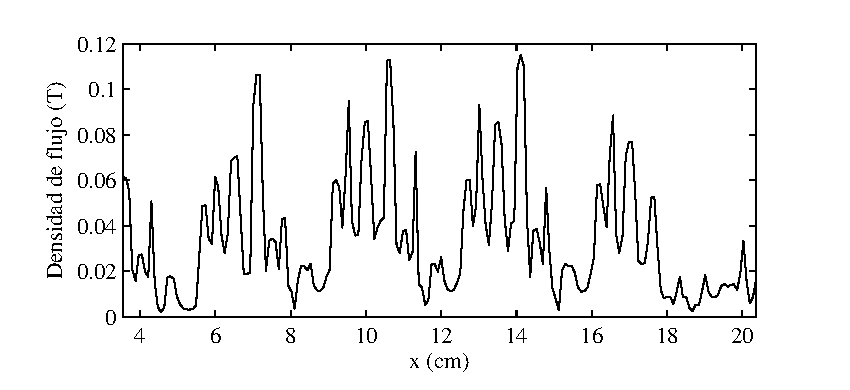
\includegraphics[scale=1]{../img/Desarrollo_de_un_diseno_inicial/airgapmfd.eps}
\caption{Densidad de flujo magnético en el entrehierro}
\label{fig:airgapmfd}
\end{figure}

Los valores obtenidos para las inductancias de los ejes directo y en cuadratura confirman esta conjetura. Los valores estimados durante el diseño se compararon con los resultados del estudio utilizando curvas de magnetización lineales y no lineales (con saturación). Esta comparación se muestra en la Tabla \ref{table:inductanceresults}.

Estos resultados muestran como el modelo utilizado en el FEM es más cercano a los valores estimados durante el proceso de diseño cuando la saturación en los materiales ferromagnéticos no se tiene en cuenta, debido a que los valores de inductancia son más cercanos. Sin embargo, una vez la saturación se incluye en el modelo, estos valores caen (principalmente la inductancia en el eje directo), aún cuando la razón $L_d/L_q$ es cercana al valor estimado. No obstante, la diferencia $L_d-L_q$ es demasiado baja para cumplir los requisitos de empuje mínimo (de acuerdo a la ecuación \ref{developedThrust}).

Las curvas de magnetización que muestran la relación entre la corriente de fase y el flujo de enlace se muestran en las Figs. \ref{fig:daxismagnetization} y \ref{fig:qaxismagnetization}, donde se muestra el punto de operación. Estas curvas muestran como el valor bajo de la inductancia en el eje directo se relacionan con la saturación debido a un incremento la corriente de magnetización en este eje.

\begin{table}[t]
\centering
\caption{Comparación de valores de $L_d$ y $L_q$ calculados según las ecuaciones y con base en el FEM.}
\label{table:inductanceresults}
\begin{tabular}{c c c c c}
\hline\hline\\
Método & $L_d$ (H) & $L_q$ (H) & $L_d/L_q$ & $L_d-L_q$ (H)\\
\hline\\
Estimados & 0.199 & 0.053 & 3.75 & 0.146\\
FEM & 0.179 & 0.038 & 4.71 & 0.141\\
FEM con saturación & 0.120 & 0.032 & 3.74 & 0.088\\
\hline\hline\\
\end{tabular}
\end{table}

\begin{figure}[hbtp]
\centering
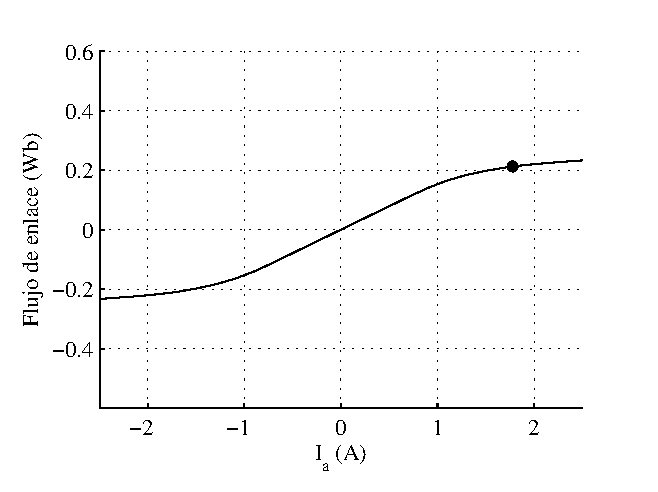
\includegraphics[scale=1]{../img/Desarrollo_de_un_diseno_inicial/daxismagnetization.eps}
\caption{Curva de magnetización en el eje directo.}
\label{fig:daxismagnetization}
\end{figure}

\begin{figure}[hbtp]
\centering
\includegraphics[scale=1]{../img/Desarrollo_de_un_diseno_inicial/qaxismagnetization.eps}
\caption{Curva de magnetización en el eje en cuadratura.}
\label{fig:qaxismagnetization}
\end{figure}

Este efecto notorio de saturación se atribuyó a la presencia de partes delgadas en el motor, debido a que, como se describió durante el procedimiento de diseño, el principal objetivo consistió en incrementar la razón $L_d/L_q$ a medida que el tamaño del primario se mantenía bajo.

\section{Mejora del diseño}
Tras observar los resultados anteriores, se procedió a mejorar el diseño suavizando las restricciones en el tamaño del motor, e incrementando los requisitos de empuje de 50 N a 80 N, repitiendo el proceso de diseño descrito anteriormente. Los parámetros obtenidos para este diseño se muestran en la Tabla \ref{table:physicalimprovedparams}. Esta tabla muestra cómo el tamaño del motor incrementó, pasando la longitud del primario de un valor de 16.9 cm a 29 cm. Esto también aplica a otros parámetros, como la altura posterior del núcleo y el ancho de las laminaciones. 

\begin{table}[t]
\centering
\caption{Parámetros físicos del diseño mejorado}
\label{table:physicalimprovedparams}
\begin{tabular}{c c c}
\hline\hline\\
Símbolo & Descripción & Valor \\
\hline\\
$\tau$ & Paso polar & 6 cm\\
$g$ & Distancia del entrehierro & 0.5 mm\\
$y/\tau$ & Razón paso de bobina/paso polar & 5/6\\
$W$ & Ancho del motor & 7.14 cm\\
$\tau_s$ & Paso de ranura & 1 cm\\
$b_s$ & Ancho de ranura & 5 mm\\
$h_s$ & Alto de ranura & 2 cm\\
$h_c$ & Altura posterior del núcleo & 1.5 cm\\
$z$ & Número de ranuras en el primario & 29\\
$W_1$ & Vueltas por fase & 456\\
$L_p$ & Longitud del primario & 29 cm\\
$w_{rr}$ & Ancho de las laminaciones & 3.75 mm\\
\hline\hline\\
\end{tabular}
\end{table}

Los resultados del análisis del nuevo diseño se muestran en la Tabla \ref{table:improvedinductanceresults}, los cuales muestran que en el diseño mejorado se presenta una razón $L_d/L_q$ más alta al igual que una diferencia entre las inductancias mayor. Estos valores producen un empuje de 50.69 N, que junto con una frecuencia de línea que produce un campo magnético viajero a una velocidad de 2 m/s, resultan en una potencia mecánica de salida de 100.3 W.

\begin{table}[btp]
\centering
\caption{Comparación de valores de $L_d$ y $L_q$ entre el diseño inicial y el mejorado}
\label{table:improvedinductanceresults}
\begin{tabular}{c c c c c}
\hline\hline\\
Método & $L_d$ (H) & $L_q$ (H) & $L_d/L_q$ & $L_d-L_q$ (H)\\
\hline\\
Diseño inicial & 0.120 & 0.032 & 3.74 & 0.088\\
Diseño mejorado & 0.203 & 0.036 & 5.64 & 0.167\\
\hline\hline\\
\end{tabular}
\end{table}

Es necesario notar que aunque los requisitos de potencia fueron cumplidos, existe una discrepancia entre los valores estimados durante el proceso de diseño y los obtenidos a partir del FEM. Esto puede verificarse al dibujar las curvas de magnetización para el diseño mejorado, como se muestra en las Figs. \ref{fig:daxismagnetization2} y \ref{fig:qaxismagnetization2}. Estas curvas muestran que, aunque el flujo fue incrementado, el motor opera en niveles más altos de saturación que en el diseño inicial, razón por la cual existen diferencias entre los valores estimados y los resultados del FEM. El hecho de que el motor opere en altos niveles de saturación durante su operación continua también se refleja durante la aceleración, ya que esta condición requiere niveles más altos de corriente que producirán mayor saturación. En general, se sabe que las máquinas de reluctancia tienden a presentar altos niveles de saturación, como se muestra en \cite{agarlita2012,boldea2015}.

\begin{figure}[hbtp]
\centering
\includegraphics[scale=1]{../img/Desarrollo_de_un_diseno_inicial/daxismagnetization2.eps}
\caption{Curva de magnetización en el eje directo.}
\label{fig:daxismagnetization2}
\end{figure}

\begin{figure}[hbtp]
\centering
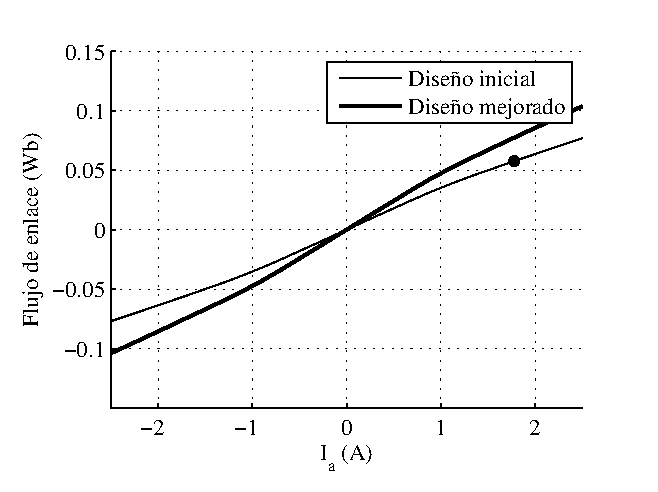
\includegraphics[scale=1]{../img/Desarrollo_de_un_diseno_inicial/qaxismagnetization2.eps}
\caption{Curva de magnetización en el eje en cuadratura.}
\label{fig:qaxismagnetization2}
\end{figure}

Una vez los requisitos de potencia han sido cumplidos, se obtuvo el empuje como función del desplazamiento, donde la fuerza es calculada de acuerdo a la ecuación \ref{developedThrust} para diferentes posiciones del primario. Estas posiciones varían desde una posición en la que el eje magnético de la fase A está completamente alineado con la posición de mayor reluctancia, hasta la posición de menor reluctancia. Los resultados se muestran en la Fig. \ref{fig:fxdata}, donde los círculos muestran las posiciones en las que se midió el empuje. De esta curva, se observa que existen valores positivos en su mayoría, pero también valores negativos de empuje, cuyo efecto combinado puede producir rizado en el movimiento, el cual es un efecto conocido en los MLR \cite{stumberger2001,yuya2007}.

\begin{figure}[hbtp]
\centering
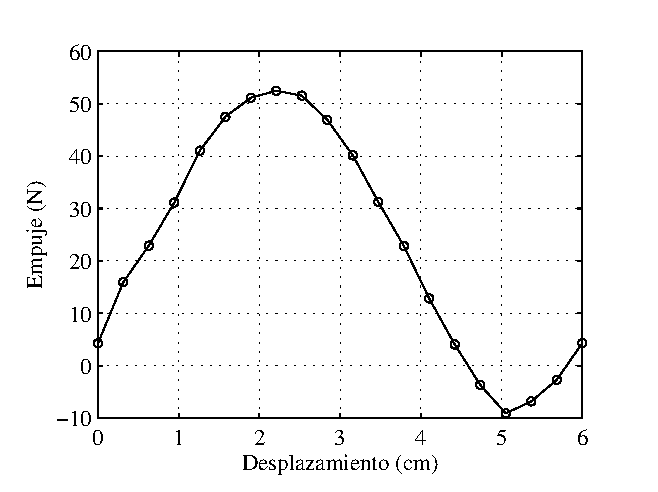
\includegraphics[scale=1]{../img/Desarrollo_de_un_diseno_inicial/fxdata.eps}
\caption{Empuje contra desplazamiento horizontal.}
\label{fig:fxdata}
\end{figure}

La resistencia del primario calculada a partir del FEM fue de 20 $\Omega$, produciendo pérdidas en el cobre de hasta 217 W para una corriente de fase de 2.7 A. Con una potencia mecánica de salida de 103 W, la eficiencia obtenida con el diseño es de 32.3\%. Este resultado es debido a que el área transversal de los cables utilizados en el devanado se calculó a partir del área disponible en cada ranura y el número de vueltas por ranura. El diseño final produjo cables con baja área transversal (con diámetros de alrededor de 0.8 mm) que contribuyen a incrementar la resistencia del primario en una cantidad considerable, incrementando las pérdidas en el cobre y disminuyendo la eficiencia del motor. Al incrementar el diámetro a 1 mm, las pérdidas en el cobre bajan a 121 W (44\% menos), aunque este diámetro no es viable teniendo en cuenta el número de vueltas por ranura.

Como se muestra en \cite{mirzaei2008,boldea2013}, el máximo factor de potencia que se puede obtener con un MLR está dado por
\begin{equation}
\cos\phi = \frac{L_d-L_q}{L_d+L_q}
\end{equation}
que para el diseño mejorado indica un valor de 0.7. 

En la Tabla \ref{table:electmechparamsfinal} se muestran las características del diseño mejorado.

\begin{table}[t]
\centering
\caption{Características eléctricas y mecánicas del diseño mejorado}
\label{table:electmechparamsfinal}
\begin{tabular}{c c c}
\hline\hline\\
Descripción & Valor \\
\hline\\
Empuje & 50.69 N\\
Aceleración & 26 m/s$^2$\\
Velocidad & 2 m/s\\
Potencia mecánica & 100.3 W\\
Voltaje de fase & 45 V\\
Corriente de fase & 2.7 A\\
Eficiencia & 32.3\%\\
Factor de potencia & 0.7\\ % Pending
\hline\hline\\
\end{tabular}
\end{table}

\section{Conclusiones}
El método expuesto utilizado para el diseño del MLR estuvo basado en relaciones entre su geometría y las especificaciones con sus medidas de desempeño, como el empuje, la eficiencia y el factor de potencia. Sin embargo, el papel del diseñador es crucial en esta metodología, ya que es necesario realizar estimaciones y suposiciones que recaen en la experiencia en el trabajo con el tipo de máquina en cuestión, cuya validez es crítica para producir un diseño que cumple los requisitos satisfactoriamente. 

Una de las prioridades durante el diseño consistió en obtener un primario pequeño, lo cual causó altos niveles de saturación para una potencia de 100 W y limitó la razón $L_d/L_q$, requiriendo corrientes de fase altas y conductores de baja sección transversal que a su vez incrementaron las pérdidas en el cobre y disminuyeron la eficiencia del motor.

Al obtener el diseño mejorado, aún cuando se observó que un incremento en el tamaño aumentó la razón $L_d/L_q$, no existe una guía clara en cuanto a cómo modificar la geometría (tanto del primario como del secundario) de forma que el desempeño del motor mejore. En el trabajo realizado, el FEM fue utilizado como herramienta de validación, que junto con un proceso iterativo que mezcló relaciones analíticas junto con la experiencia, produjo un diseño que cumplió con los requisitos de potencia establecidos, pero con una eficiencia menor al 40\%.

Como alternativa, puede utilizarse una metodología de diseño acoplada con el FEM para guiar la definición de los parámetros del motor \cite{hasanien2010}. Por otro lado, el diseño obtenido se puede utilizar como un diseño inicial para proceder con un método de optimización que reduzca la dependencia en la experiencia del diseñador y que, junto con el FEM, produza un diseño más confiable y eficiente.

\bibliographystyle{ieeetr}
\bibliography{../refs}
